\chapter{Implementation}


\section{Structure of project-folder}
The project can be downloaded from \url{https://github.com/renbem/RCCPP-coursework02}. The code is structured in several folders within the main directory:
\begin{itemize}
	\item \texttt{documentation:} Contains all documentation of the project including this report and the code documentation generated by doxygen\footnote{\url{www.doxygen.org}}.
	\item \texttt{include:} Contains all header files (\texttt{*.h})
	\item \texttt{matlab:} Contains the \textsc{Matlab}-files used for the random generation of initial boards (or grid according to the terminology in chapter 1), the creation of the Game of Life video\footnote{Provided at \url{https://www.youtube.com/watch?v=AeIm2I_9n5g&feature=youtu.be}} and statistical evaluation of the results.
	\item \texttt{source:} Contains the code files (\texttt{*.cc}).
	\item \texttt{test:}  Contains all data and source files for the unit tests.
\end{itemize}

\section{Choice of design}
The implementation follows the design as illustrated in \cref{fig:OverviewOfImplementation} which translates the concept of a having a game consisting of boards which in turn consist of the cells.

The classes are designed so that a new iteration is triggered by the member function \texttt{computeNextStep} of \texttt{Game}, cf. \cref{fig:computeNextStepCall}. I decided to connect the "rules of the game" with the board via the two methods \texttt{determineNeighbourCells} and \texttt{applyTransitionRules}. One could argue that this might be better situated in the class \texttt{Game} since the rules can be considered as an intrinsic property of the game and the board could be of arbitrary shape. However, since the Conway's Game of Life relies on well-established rules in order to have a "meaningful game" (i.e. no extinction or overcrowding of cells) the definition of a neighbour and the propagation rules depend strongly on the shape and therefore on the board.

\begin{figure}
	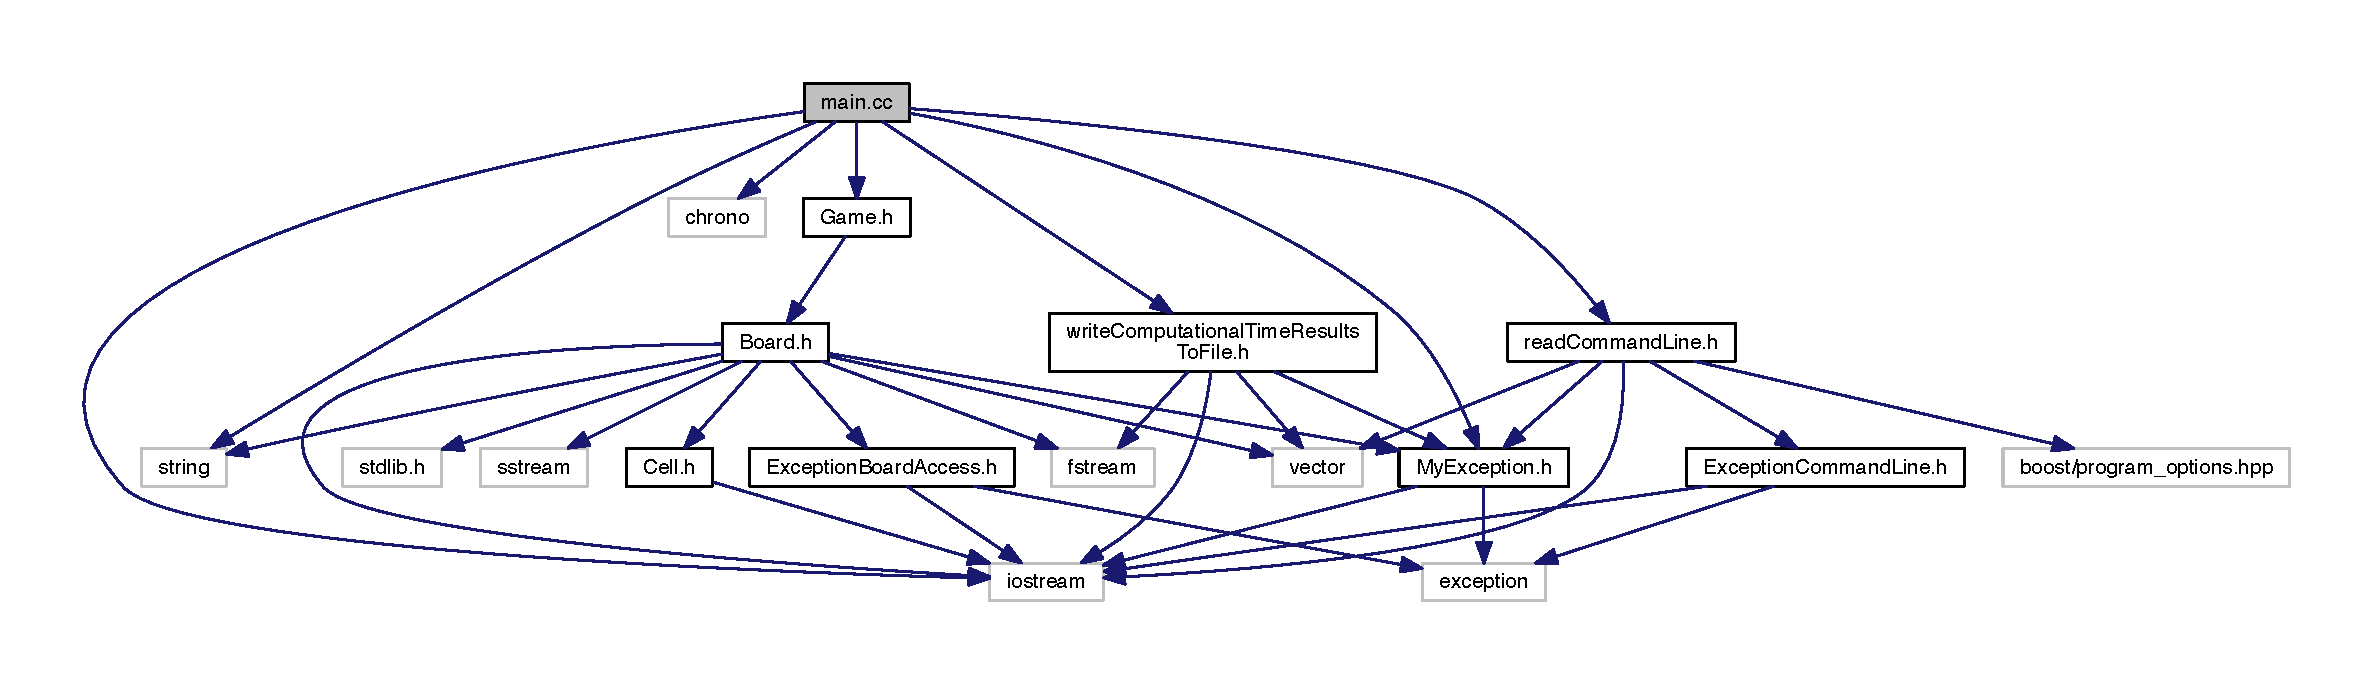
\includegraphics[width=\textwidth]{doxygen/latex/a00143.pdf}
	\caption{Overview of implementation}
	\label{fig:OverviewOfImplementation}
\end{figure}


\begin{figure}
	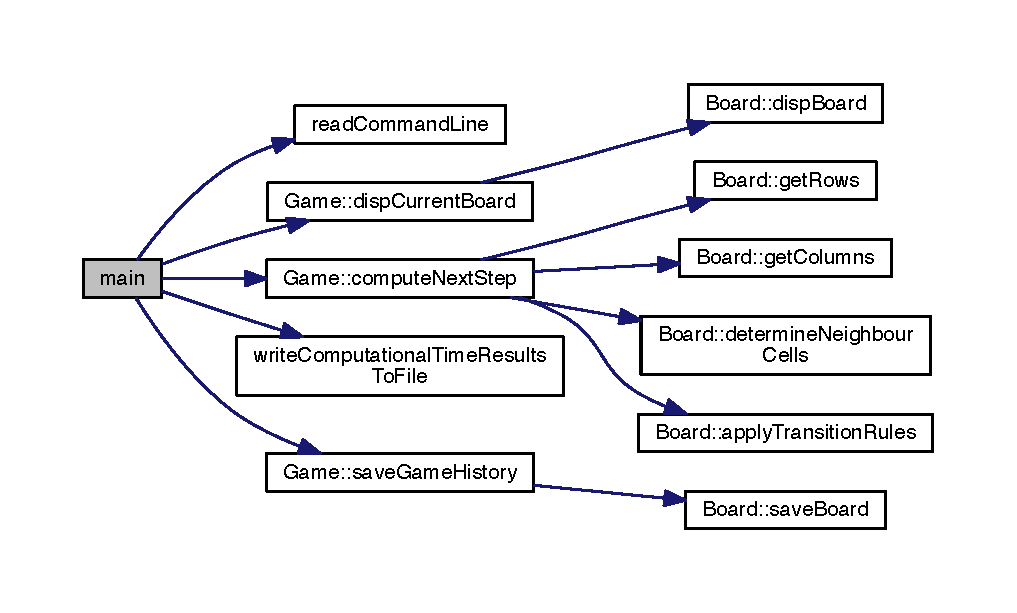
\includegraphics[width=\textwidth]{doxygen/latex/a00108_a3c04138a5bfe5d72780bb7e82a18e627_cgraph.pdf}
	\caption{Call graph of \texttt{main.cc}}
	\label{fig:computeNextStepCall}
\end{figure}

%It was aimed that a minimal amount of methods are defined as public to fulfil their purpose. The public methods of these three classes are illustrated in \cref{fig:MainClasses}.
%
%\begin{figure}\centering
%	\subfloat[\texttt{Game}]{\label{fig:Game}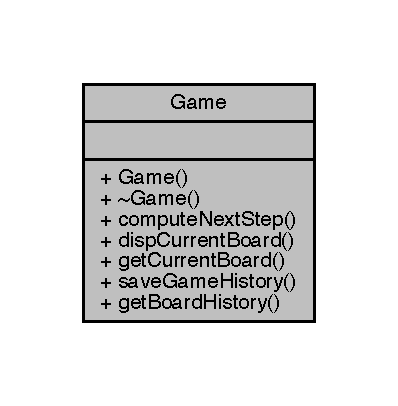
\includegraphics[width=0.33\textwidth]{doxygen/latex/a00165.pdf}}
%	\subfloat[\texttt{Board}]{\label{fig:Board}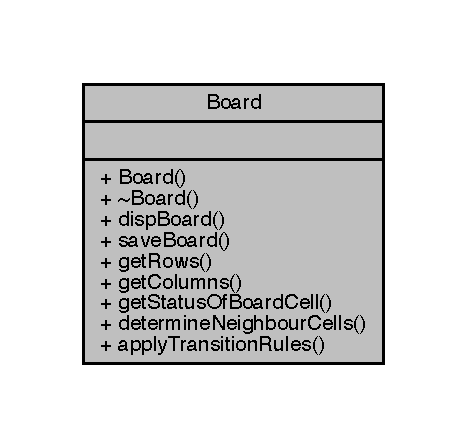
\includegraphics[width=0.33\textwidth]{doxygen/latex/a00155.pdf}}
%	\subfloat[\texttt{Cell}]{\label{fig:Cell}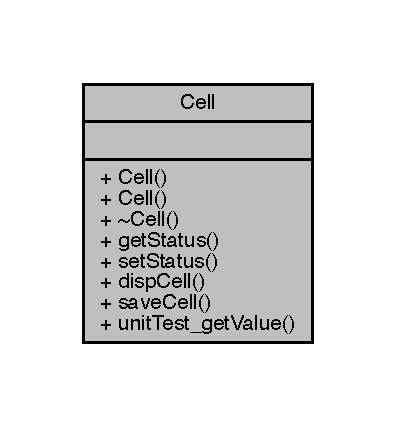
\includegraphics[width=0.33\textwidth]{doxygen/latex/a00157.pdf}}
%	\caption{Main classes of implementation and their public methods}
%	\label{fig:MainClasses}
%\end{figure}

\subsection{Parallelisation}
The code was parallelised via \textbf{OpenMP} within the method \texttt{computeNextStep}, cf. line 10 in \cref{Gamecc}. The line 9 and 11 was added since I could not compile it without any error messages on Mac (further instructions in \cref{sec:BuildRunTest}) but it works on Ubuntu. Therefore, the code runs on non-linux platforms only in the serial version.


\lstinputlisting
[style=myCppStyle,caption={Game::computeNextStep},label=Gamecc,belowskip=7mm,frame=lines,linerange={29-49}]
{../source/Game.cc}

\subsection{Unit tests}
Unit tests were written to test the following cases:
\begin{itemize}
	\item Check input file\footnote{It is only tested whether the input file exists. Many other cases should be tested in addition. E.g.: Format of file appropriate?, Number of columns always identical?, Minimum number of rows and columns alright? etc.}.
	\item Several tests to check malformed command lines.
	\item Several tests to check whether the correct neighbours are returned by \texttt{Board::neighbourCells}. (The "infinite board" was implemented by assuming periodic boundary conditions.)
	\item Attempted access to non-existing indices of board throws an exception.
	\item Test whether one step of Conway's Game of Life is computed correctly.
	\item Test whether the parallel computation via OpenMP returns the same board as the serial version.
	
\end{itemize}
The respective file \texttt{main\_UnitTests.cc} is located in \texttt{test/}

\section{Build, run and test}\label{sec:BuildRunTest}
The respective \texttt{CMakeLists.txt} file in the parent directory to build the code was tested on two operating systems:

\begin{itemize}
	\item OS X 10.10.3 (Macbook Pro, 2.5 GHz Intel Core i7)
	\item Ubuntu 14.04 (Virtual machine via VirtualBox\footnote{\url{https://www.virtualbox.org/}} within OS X 10.10.3)
\end{itemize}

Unfortunately, I couldn't run OpenMP on Mac without any errors (comments are provided in the \texttt{CMakeLists.txt} file). Therefore, I used VirtualBox to build it on Ubuntu where everything went without any problems. Consequently, I configured the CMake file (and added the respective lines in \texttt{Game.cc}) so that the code runs on Mac in serial and on Ubuntu with OpenMP. The results in \cref{sec:results} are based on the computation in Ubuntu.


\subsection{Build instructions}
In order to build the code run the following lines in the main directory:
\begin{quote}
	\texttt{mkdir build}\\
	\texttt{cd build}\\
	\texttt{cmake ..}\\
	\texttt{make}
\end{quote}


After building the code two binary files will be generated:
\begin{itemize}
	\item \texttt{conwaysGameOfLife} located in \texttt{build/test/bin/}
	\item \texttt{conwaysGameOfLife\_UnitTests} located in \texttt{build/test/bin/}
\end{itemize}


\subsection{Running the programme}
For running the code several example data sets are provided in \texttt{build/test/exampleData/}.
A possible command of the programme within the \texttt{build}-folder reads
\begin{quote}
	\texttt{bin/conwaysGameOfLife -{}-i "test/exampleData/InitialBoardRandom\_10Times10.txt" -{}-o "out\_BoardHistory.txt" -{}-s 100}
\end{quote}
which uses the initial board defined in \texttt{InitialBoardRandom\_10Times10.txt} and performs 100 steps by applying the transition rules given in \cref{table:rules}. A concatenated history of all computed boards is then stored in \texttt{out\_BoardHistory.txt} and the information of the corresponding computational time per iteration is saved in \texttt{out\_BoardHistory\_ComputationalTime.txt}.
Alternatively any other file \texttt{InitialBoardRandom\_*.txt} in \texttt{test/exampleData} can be used as input file\footnote{A "on-screen-simulation" and its corresponding computational time can also be enabled by setting the respective flags \texttt{flagDisplayGame} and \texttt{flagDisplayComputationalTime} to \texttt{true} within \texttt{main.cc}.}.

\subsection{Run unit tests}
To run the unit tests, execute the command
\begin{quote}
	\texttt{./conwaysGameOfLife\_UnitTest}
\end{quote}
in \texttt{build/test/bin/}.


\section{Results}\label{sec:results}

\begin{figure}\centering
	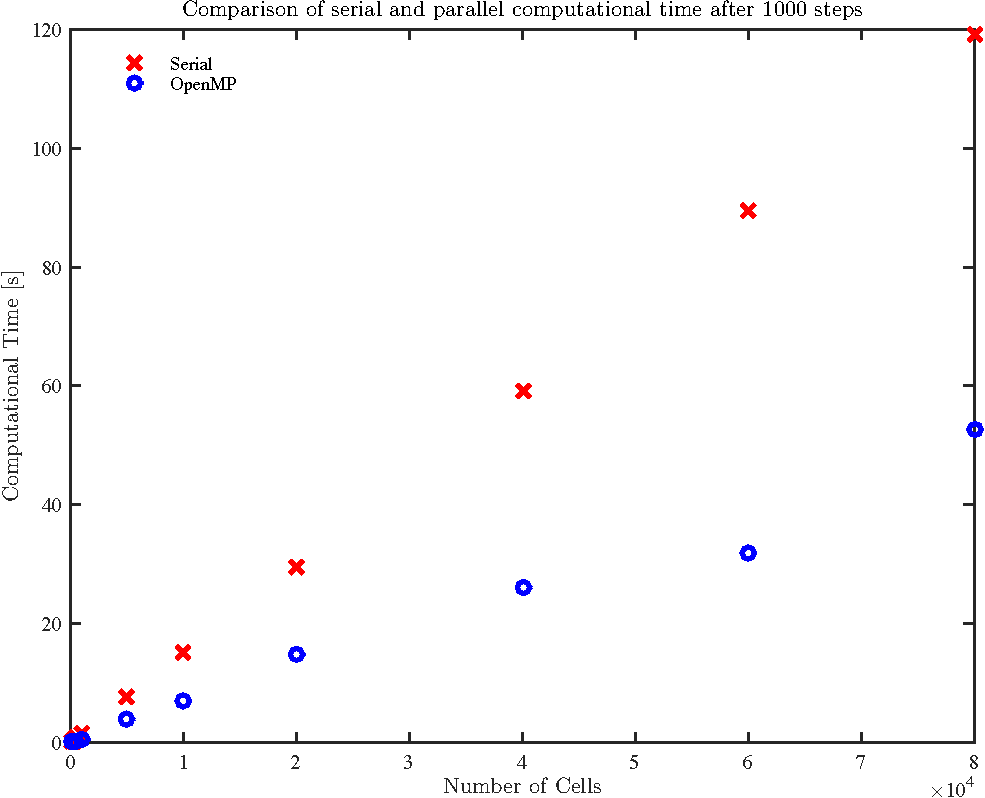
\includegraphics[width=0.8\textwidth]{figures/SerialOpenMP_Cells.pdf}
	\caption{Computational time over number of cells}
\end{figure}

\begin{figure}\centering
	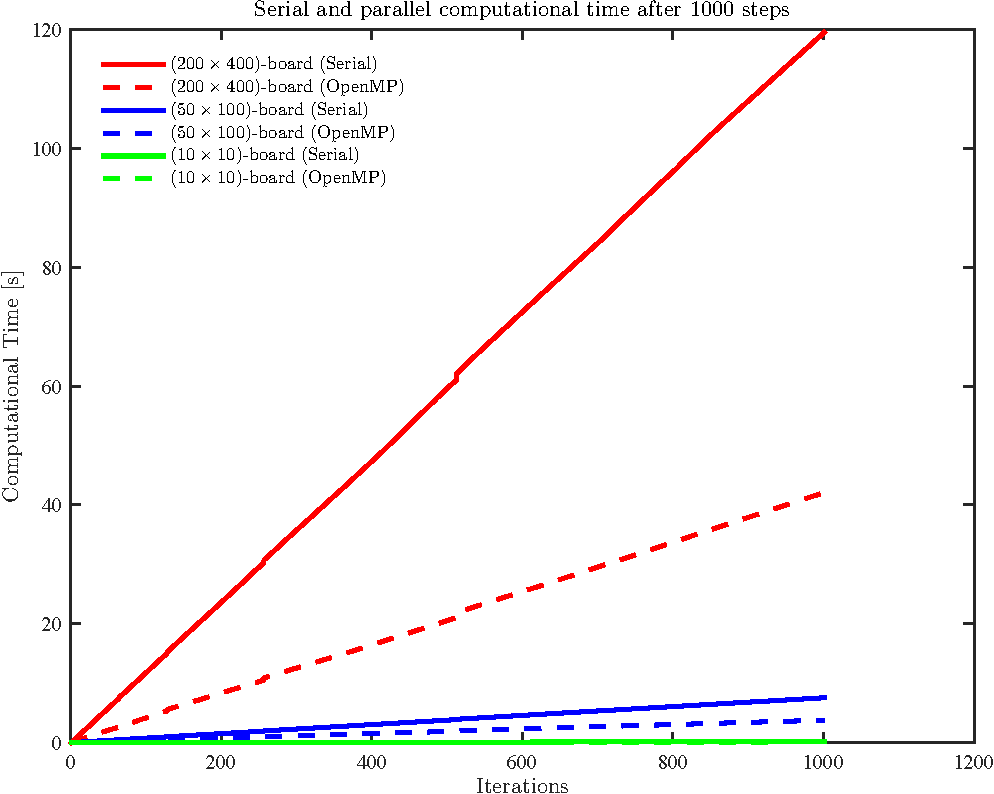
\includegraphics[width=0.8\textwidth]{figures/SerialOpenMP_Iterations.pdf}
	\caption{Computational time over number of iterations}
\end{figure}

\begin{figure}\centering
	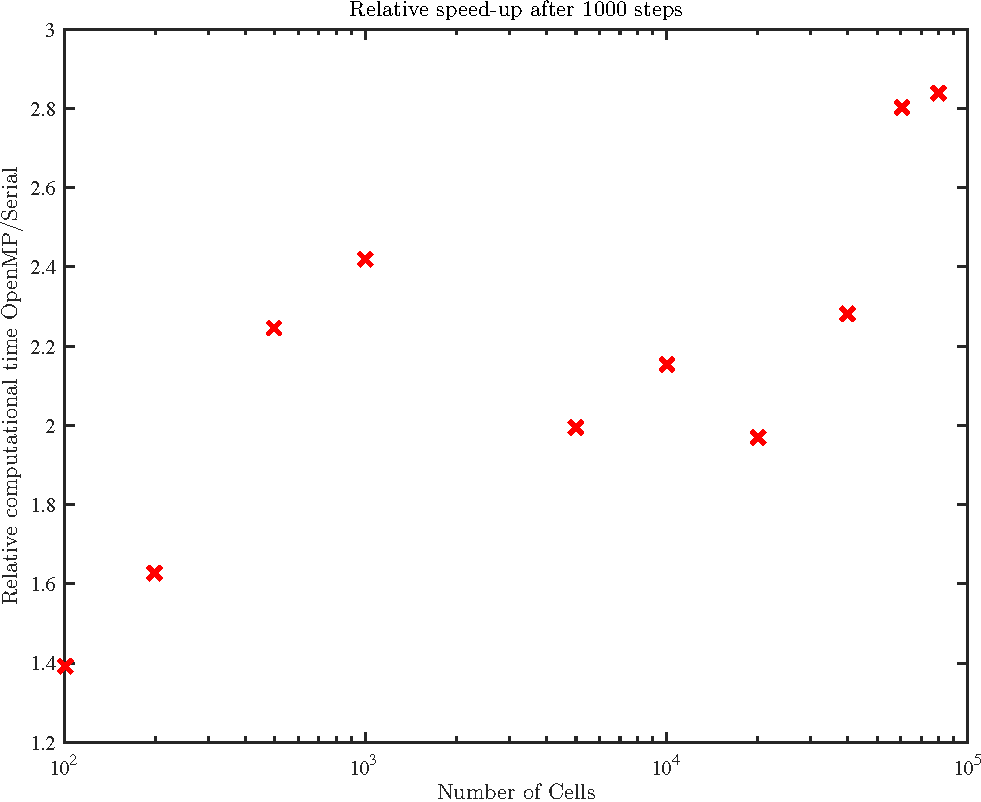
\includegraphics[width=0.8\textwidth]{figures/SerialOpenMP_Speedup.pdf}
	\caption{Relative speed-up}
\end{figure}